\documentclass{extbook}[14pt]
\usepackage{multicol, enumerate, enumitem, hyperref, color, soul, setspace, parskip, fancyhdr, amssymb, amsthm, amsmath, latexsym, units, mathtools}
\everymath{\displaystyle}
\usepackage[headsep=0.5cm,headheight=0cm, left=1 in,right= 1 in,top= 1 in,bottom= 1 in]{geometry}
\usepackage{dashrule}  % Package to use the command below to create lines between items
\newcommand{\litem}[1]{\item #1

\rule{\textwidth}{0.4pt}}
\pagestyle{fancy}
\lhead{}
\chead{Answer Key for Progress Quiz 6 Version A}
\rhead{}
\lfoot{1430-1829}
\cfoot{}
\rfoot{test}
\begin{document}
\textbf{This key should allow you to understand why you choose the option you did (beyond just getting a question right or wrong). \href{https://xronos.clas.ufl.edu/mac1105spring2020/courseDescriptionAndMisc/Exams/LearningFromResults}{More instructions on how to use this key can be found here}.}

\textbf{If you have a suggestion to make the keys better, \href{https://forms.gle/CZkbZmPbC9XALEE88}{please fill out the short survey here}.}

\textit{Note: This key is auto-generated and may contain issues and/or errors. The keys are reviewed after each exam to ensure grading is done accurately. If there are issues (like duplicate options), they are noted in the offline gradebook. The keys are a work-in-progress to give students as many resources to improve as possible.}

\rule{\textwidth}{0.4pt}

\begin{enumerate}\litem{
Determine the domain of the function below.
\[ f(x) = \frac{5}{18x^{2} -39 x + 20} \]The solution is \( \text{All Real numbers except } x = 0.833 \text{ and } x = 1.333. \), which is option D.\begin{enumerate}[label=\Alph*.]
\item \( \text{All Real numbers except } x = a, \text{ where } a \in [11.91, 12.04] \)

All Real numbers except $x = 12.000$, which corresponds to removing a distractor value from the denominator.
\item \( \text{All Real numbers except } x = a, \text{ where } a \in [0.74, 0.97] \)

All Real numbers except $x = 0.833$, which corresponds to removing only 1 value from the denominator.
\item \( \text{All Real numbers.} \)

This corresponds to thinking the denominator has complex roots or that rational functions have a domain of all Real numbers.
\item \( \text{All Real numbers except } x = a \text{ and } x = b, \text{ where } a \in [0.74, 0.97] \text{ and } b \in [1.28, 1.61] \)

All Real numbers except $x = 0.833$ and $x = 1.333$, which is the correct option.
\item \( \text{All Real numbers except } x = a \text{ and } x = b, \text{ where } a \in [11.91, 12.04] \text{ and } b \in [29.82, 30.39] \)

All Real numbers except $x = 12.000$ and $x = 30.000$, which corresponds to not factoring the denominator correctly.
\end{enumerate}

\textbf{General Comment:} Recall that dividing by zero is not a real number. Therefore the domain is all real numbers \textbf{except} those that make the denominator 0.
}
\litem{
Solve the rational equation below. Then, choose the interval(s) that the solution(s) belongs to.
\[ \frac{-80}{-40x -60} + 1 = \frac{-80}{-40x -60} \]The solution is \( \text{all solutions are invalid or lead to complex values in the equation.} \), which is option A.\begin{enumerate}[label=\Alph*.]
\item \( \text{All solutions lead to invalid or complex values in the equation.} \)

*$x = -1.500$ leads to dividing by 0 in the original equation and thus is not a valid solution, which is the correct option.
\item \( x \in [-1.5,-0.5] \)

$x = -1.500$, which corresponds to not checking if this value leads to dividing by 0 in the original equation and thus is not a valid solution.
\item \( x_1 \in [-1.5, 0.5] \text{ and } x_2 \in [-2.5,0.5] \)

$x = -1.500 \text{ and } x = -1.500$, which corresponds to getting the correct solution and believing there should be a second solution to the equation.
\item \( x_1 \in [-1.5, 0.5] \text{ and } x_2 \in [0.5,2.5] \)

$x = -1.500 \text{ and } x = 1.500$, which corresponds to getting the correct solution and believing there should be a second solution to the equation.
\item \( x \in [0.5,3.5] \)

$x = 1.500$, which corresponds to not distributing the factor $-40x -60$ correctly when trying to eliminate the fraction.
\end{enumerate}

\textbf{General Comment:} Distractors are different based on the number of solutions. Remember that after solving, we need to make sure our solution does not make the original equation divide by zero!
}
\litem{
Solve the rational equation below. Then, choose the interval(s) that the solution(s) belongs to.
\[ \frac{2x + 0}{6x + 3} + \frac{-4x^{2} +0 x + 0}{-18x^{2} -33 x -12} = \frac{-2}{-3x -4} \]The solution is \( \text{There are two solutions: } x = -0.600 \text{ and } x = 1.000 \), which is option A.\begin{enumerate}[label=\Alph*.]
\item \( x_1 \in [-0.99, 0.35] \text{ and } x_2 \in [0.5,1.1] \)

* $x = -0.600 \text{ and } x = 1.000$, which is the correct option.
\item \( x_1 \in [-0.99, 0.35] \text{ and } x_2 \in [-2,0.8] \)


\item \( x \in [-0.53,1.82] \)


\item \( \text{All solutions lead to invalid or complex values in the equation.} \)


\item \( x \in [-1.43,-0.7] \)


\end{enumerate}

\textbf{General Comment:} Distractors are different based on the number of solutions. Remember that after solving, we need to make sure our solution does not make the original equation divide by zero!
}
\litem{
Determine the domain of the function below.
\[ f(x) = \frac{6}{15x^{2} -3 x -12} \]The solution is \( \text{All Real numbers except } x = -0.800 \text{ and } x = 1.000. \), which is option B.\begin{enumerate}[label=\Alph*.]
\item \( \text{All Real numbers.} \)

This corresponds to thinking the denominator has complex roots or that rational functions have a domain of all Real numbers.
\item \( \text{All Real numbers except } x = a \text{ and } x = b, \text{ where } a \in [-2.1, 0.2] \text{ and } b \in [0.2, 2.2] \)

All Real numbers except $x = -0.800$ and $x = 1.000$, which is the correct option.
\item \( \text{All Real numbers except } x = a, \text{ where } a \in [-21.1, -19.6] \)

All Real numbers except $x = -20.000$, which corresponds to removing a distractor value from the denominator.
\item \( \text{All Real numbers except } x = a \text{ and } x = b, \text{ where } a \in [-21.1, -19.6] \text{ and } b \in [8.7, 9.5] \)

All Real numbers except $x = -20.000$ and $x = 9.000$, which corresponds to not factoring the denominator correctly.
\item \( \text{All Real numbers except } x = a, \text{ where } a \in [-2.1, 0.2] \)

All Real numbers except $x = -0.800$, which corresponds to removing only 1 value from the denominator.
\end{enumerate}

\textbf{General Comment:} Recall that dividing by zero is not a real number. Therefore the domain is all real numbers \textbf{except} those that make the denominator 0.
}
\litem{
Choose the equation of the function graphed below.

\begin{center}
    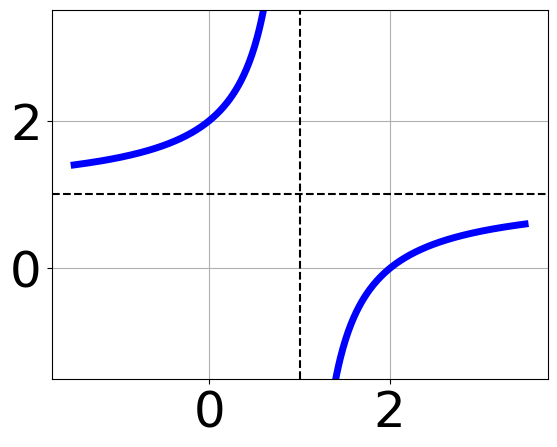
\includegraphics[width=0.5\textwidth]{../Figures/rationalGraphToEquationCopyA.png}
\end{center}


The solution is \( \text{None of the above as it should be } f(x) = \frac{1}{x - 1} + 3 \), which is option E.\begin{enumerate}[label=\Alph*.]
\item \( f(x) = \frac{1}{x + 1} + 7 \)

The $x$- and $y$-value of the equation does not match the graph.
\item \( f(x) = \frac{1}{(x + 1)^2} + 7 \)

Corresponds to thinking the graph was a shifted version of $\frac{1}{x^2}$ not noticing the $y$-value was wrong.
\item \( f(x) = \frac{-1}{x - 1} + 7 \)

Corresponds to using the general form $f(x) = \frac{a}{x-h}+k$, the opposite leading coefficient AND not noticing the $y$-value was wrong.
\item \( f(x) = \frac{-1}{(x - 1)^2} + 7 \)

Corresponds to thinking the graph was a shifted version of $\frac{1}{x^2}$, using the general form $f(x) = \frac{a}{x-h}+k$, the opposite leading coefficient, AND not noticing the $y$-value was wrong.
\item \( \text{None of the above} \)

None of the equation options were the correct equation.
\end{enumerate}

\textbf{General Comment:} Remember that the general form of a basic rational equation is $ f(x) = \frac{a}{(x-h)^n} + k$, where $a$ is the leading coefficient (and in this case, we assume is either $1$ or $-1$), $n$ is the degree (in this case, either $1$ or $2$), and $(h, k)$ is the intersection of the asymptotes.
}
\litem{
Choose the graph of the equation below.
\[ f(x) = \frac{-1}{x - 2} - 3 \]The solution is the graph below, which is option A.
\begin{center}
    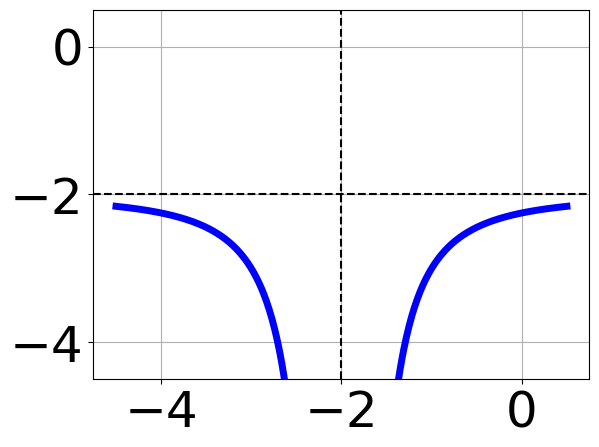
\includegraphics[width=0.3\textwidth]{../Figures/rationalEquationToGraphAA.png}
\end{center}\begin{enumerate}[label=\Alph*.]
\begin{multicols}{2}
\item 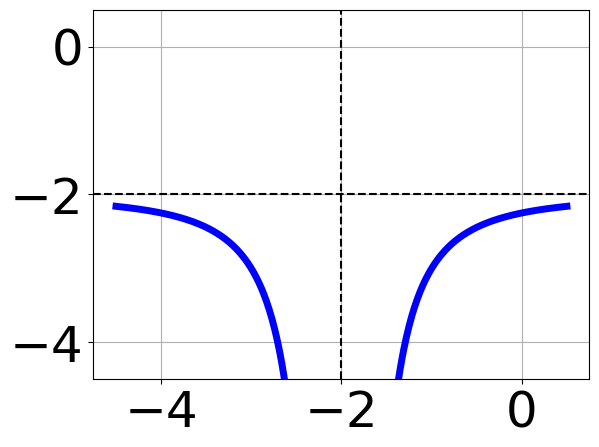
\includegraphics[width = 0.3\textwidth]{../Figures/rationalEquationToGraphAA.png}
\item 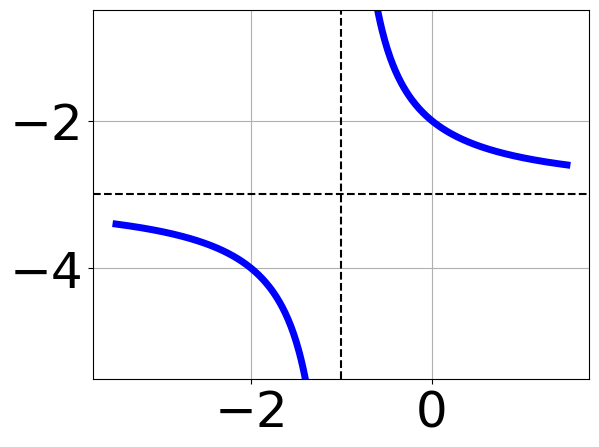
\includegraphics[width = 0.3\textwidth]{../Figures/rationalEquationToGraphBA.png}
\item 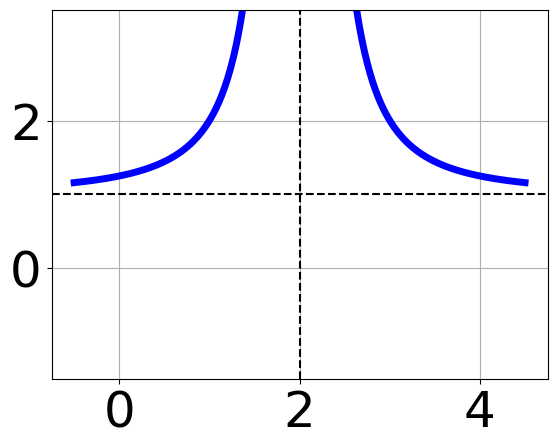
\includegraphics[width = 0.3\textwidth]{../Figures/rationalEquationToGraphCA.png}
\item 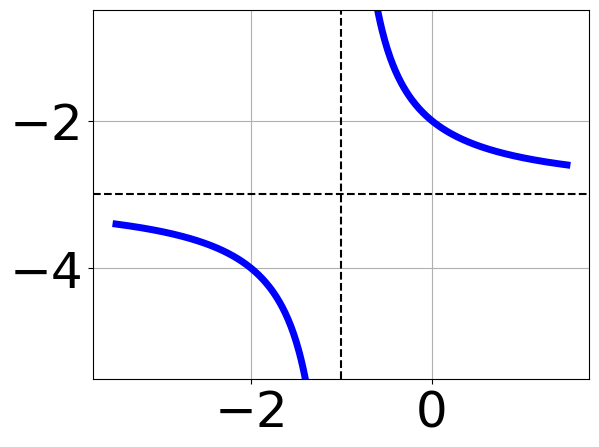
\includegraphics[width = 0.3\textwidth]{../Figures/rationalEquationToGraphDA.png}
\end{multicols}\item None of the above.\end{enumerate}
\textbf{General Comment:} Remember that the general form of a basic rational equation is $ f(x) = \frac{a}{(x-h)^n} + k$, where $a$ is the leading coefficient (and in this case, we assume is either $1$ or $-1$), $n$ is the degree (in this case, either $1$ or $2$), and $(h, k)$ is the intersection of the asymptotes.
}
\litem{
Solve the rational equation below. Then, choose the interval(s) that the solution(s) belongs to.
\[ \frac{-117}{117x + 78} + 1 = \frac{-117}{117x + 78} \]The solution is \( \text{all solutions are invalid or lead to complex values in the equation.} \), which is option D.\begin{enumerate}[label=\Alph*.]
\item \( x_1 \in [-1.1, 0.2] \text{ and } x_2 \in [0.3,1] \)

$x = -0.667 \text{ and } x = 0.667$, which corresponds to getting the correct solution and believing there should be a second solution to the equation.
\item \( x_1 \in [-1.1, 0.2] \text{ and } x_2 \in [-2.3,-0.3] \)

$x = -0.667 \text{ and } x = -0.667$, which corresponds to getting the correct solution and believing there should be a second solution to the equation.
\item \( x \in [-0.67,1.33] \)

$x = -0.667$, which corresponds to not checking if this value leads to dividing by 0 in the original equation and thus is not a valid solution.
\item \( \text{All solutions lead to invalid or complex values in the equation.} \)

*$x = -0.667$ leads to dividing by 0 in the original equation and thus is not a valid solution, which is the correct option.
\item \( x \in [-0.6,1.5] \)

$x = 0.667$, which corresponds to not distributing the factor $117x + 78$ correctly when trying to eliminate the fraction.
\end{enumerate}

\textbf{General Comment:} Distractors are different based on the number of solutions. Remember that after solving, we need to make sure our solution does not make the original equation divide by zero!
}
\litem{
Choose the graph of the equation below.
\[ f(x) = \frac{1}{(x + 2)^2} + 3 \]The solution is the graph below, which is option C.
\begin{center}
    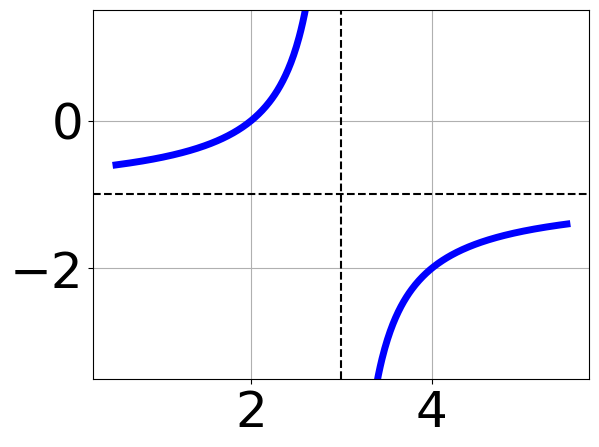
\includegraphics[width=0.3\textwidth]{../Figures/rationalEquationToGraphCopyCA.png}
\end{center}\begin{enumerate}[label=\Alph*.]
\begin{multicols}{2}
\item 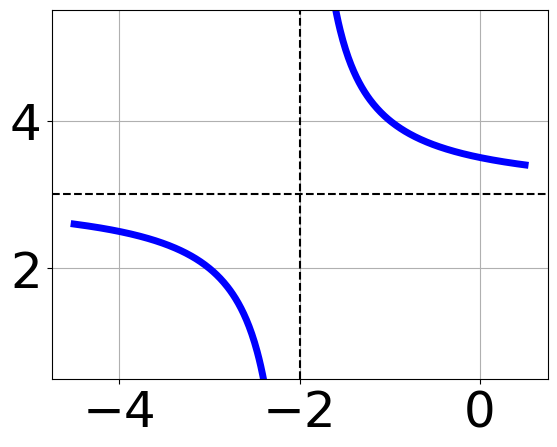
\includegraphics[width = 0.3\textwidth]{../Figures/rationalEquationToGraphCopyAA.png}
\item 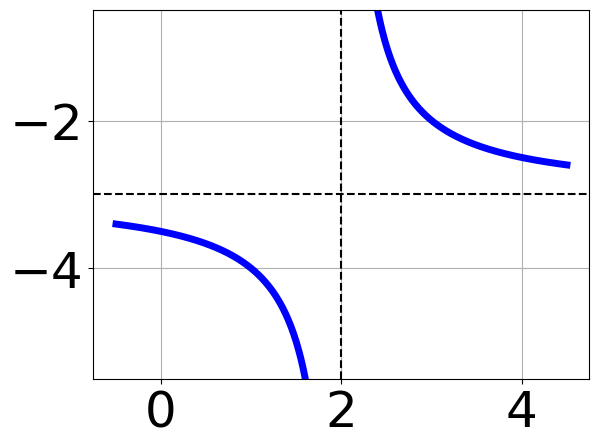
\includegraphics[width = 0.3\textwidth]{../Figures/rationalEquationToGraphCopyBA.png}
\item 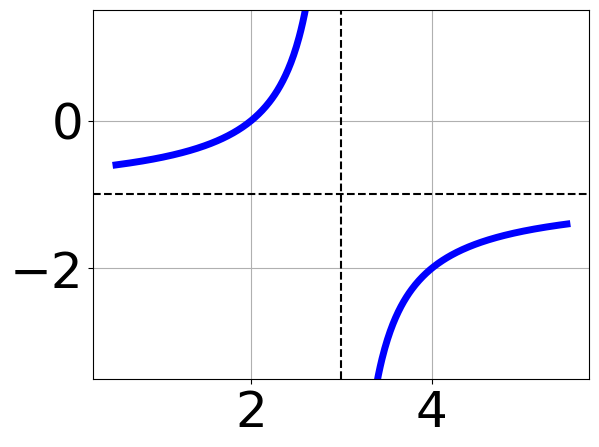
\includegraphics[width = 0.3\textwidth]{../Figures/rationalEquationToGraphCopyCA.png}
\item 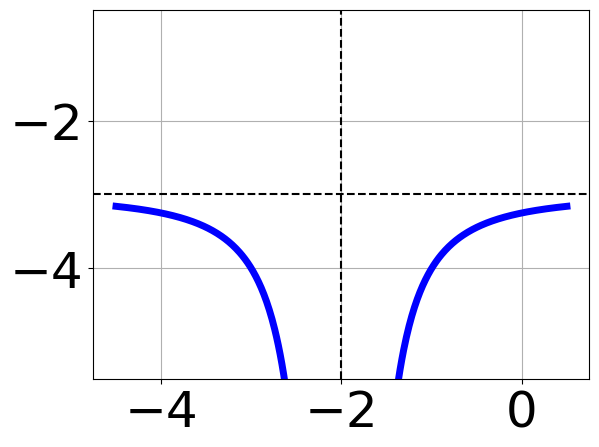
\includegraphics[width = 0.3\textwidth]{../Figures/rationalEquationToGraphCopyDA.png}
\end{multicols}\item None of the above.\end{enumerate}
\textbf{General Comment:} Remember that the general form of a basic rational equation is $ f(x) = \frac{a}{(x-h)^n} + k$, where $a$ is the leading coefficient (and in this case, we assume is either $1$ or $-1$), $n$ is the degree (in this case, either $1$ or $2$), and $(h, k)$ is the intersection of the asymptotes.
}
\litem{
Choose the equation of the function graphed below.

\begin{center}
    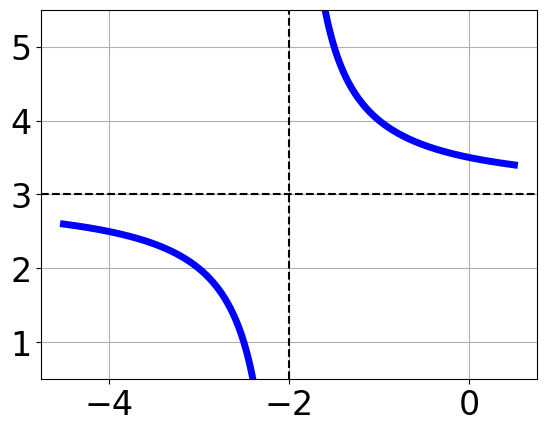
\includegraphics[width=0.5\textwidth]{../Figures/rationalGraphToEquationA.png}
\end{center}


The solution is \( f(x) = \frac{-1}{x - 1} - 2 \), which is option C.\begin{enumerate}[label=\Alph*.]
\item \( f(x) = \frac{1}{x + 1} - 2 \)

Corresponds to using the general form $f(x) = \frac{a}{x+h}+k$ and the opposite leading coefficient.
\item \( f(x) = \frac{1}{(x + 1)^2} - 2 \)

Corresponds to thinking the graph was a shifted version of $\frac{1}{x^2}$, using the general form $f(x) = \frac{a}{x+h}+k$, and the opposite leading coefficient.
\item \( f(x) = \frac{-1}{x - 1} - 2 \)

This is the correct option.
\item \( f(x) = \frac{-1}{(x - 1)^2} - 2 \)

Corresponds to thinking the graph was a shifted version of $\frac{1}{x^2}$.
\item \( \text{None of the above} \)

This corresponds to believing the vertex of the graph was not correct.
\end{enumerate}

\textbf{General Comment:} Remember that the general form of a basic rational equation is $ f(x) = \frac{a}{(x-h)^n} + k$, where $a$ is the leading coefficient (and in this case, we assume is either $1$ or $-1$), $n$ is the degree (in this case, either $1$ or $2$), and $(h, k)$ is the intersection of the asymptotes.
}
\litem{
Solve the rational equation below. Then, choose the interval(s) that the solution(s) belongs to.
\[ \frac{6x + 0}{-5x -5} + \frac{-2x^{2} +0 x + 0}{-10x^{2} +25 x + 35} = \frac{2}{2x -7} \]The solution is \( \text{There are two solutions: } x = 0.351 \text{ and } x = 2.849 \), which is option E.\begin{enumerate}[label=\Alph*.]
\item \( \text{All solutions lead to invalid or complex values in the equation.} \)


\item \( x_1 \in [0.14, 0.96] \text{ and } x_2 \in [-2.4,0.9] \)


\item \( x \in [2.86,3.56] \)


\item \( x \in [2.1,3.45] \)


\item \( x_1 \in [0.14, 0.96] \text{ and } x_2 \in [1.5,3.2] \)

* $x = 0.351 \text{ and } x = 2.849$, which is the correct option.
\end{enumerate}

\textbf{General Comment:} Distractors are different based on the number of solutions. Remember that after solving, we need to make sure our solution does not make the original equation divide by zero!
}
\end{enumerate}

\end{document}